\chapter{Results}\label{ch:results}

\begin{guide}
About 10--12 pages. Report what happened, in the order of the hypotheses, and keep interpretation short - the ``why'' goes in \cref{ch:discussion}. Every number in the tables below was copied from \texttt{Code/results/*.md} and \texttt{HANDOFF.md}; if you rerun anything, update them from those files. Every result is the mean $\pm$ std over 5 seeds unless stated. For each table or figure, write 1--2 paragraphs: what it shows, the key number, and which hypothesis it bears on.
\end{guide}

% ---------------------------------------------------------------------
\section{Return forecasting (H1, H2)}\label{sec:res-forecast}

\begin{table}[ht]
  \centering
  \caption{Next-day BTC log-return forecasts on the 2025 test set (mean $\pm$ std over 5 seeds). Naive ``no change'' MAPE: 1.7849\%.}
  \label{tab:phase2}
  \begin{tabular}{llcc}
    \toprule
    Model & Inputs & RMSE & MAPE (\%) \\
    \midrule
    Vanilla LSTM     & univariate   & 0.02337 $\pm$ 0.00005 & 1.7755 $\pm$ 0.0053 \\
    Vanilla GRU      & univariate   & 0.02348 $\pm$ 0.00019 & 1.7829 $\pm$ 0.0166 \\
    Standard Bi-LSTM & multivariate & 0.02689 $\pm$ 0.00445 & 2.1037 $\pm$ 0.4328 \\
    Alpha Agent      & multivariate & 0.02372 $\pm$ 0.00051 & 1.8160 $\pm$ 0.0421 \\
    \bottomrule
  \end{tabular}
\end{table}

\begin{guide}
Point to make: every model sits at about the naive baseline - next-day returns are close to a random walk (the Phase 1 EDA persistence $R^2$ was $-1.055$). The Bi-LSTM's poor average is one unstable seed (RMSE 0.0356).
\end{guide}

\subsection{H1: multivariate versus univariate}
\begin{guide}
Clean test: same Bi-LSTM architecture, 19 features versus BTC returns alone. Multivariate RMSE $0.02689 \pm 0.00445$ vs univariate $0.03355 \pm 0.00983$. DM tests significant on 4 of 5 seeds but split 2--2 in direction. Conclusion: directionally supported on average, not a clean or consistent result. (The Alpha-vs-LSTM comparison is NOT a clean H1 test - the architectures differ.)
\end{guide}
\tbc{}

\subsection{H2: attention versus no attention}
\begin{guide}
Alpha Agent vs Standard Bi-LSTM, identical inputs. 2 of 5 seeds significant, both in favour of attention, and both are the seeds where the Bi-LSTM trained unstably. Conclusion: attention helps when training is unstable; otherwise a small, non-significant edge. Inside the trading framework attention made no measurable difference (\cref{tab:model-ablation}).
\end{guide}
\tbc{}

% ---------------------------------------------------------------------
\section{Direction: is it predictable at all?}\label{sec:res-direction}

\begin{table}[ht]
  \centering
  \caption{Next-day direction hit rate with 95\% Wilson intervals. No rule is trained or tuned.}
  \label{tab:direction}
  \small
  \begin{tabular}{lcccc}
    \toprule
    Method & 2024 (val) & 2025 (test) & 2026 (forward) & Pooled \\
    \midrule
    Alpha Agent (5-seed avg) & 49.9\% & 51.4\% & 49.3\% & 50.2\% [46, 54] \\
    Always up                & 49.3\% & 50.2\% & 47.4\% & 49.0\% [45, 53] \\
    Momentum 1d              & 43.3\% & 43.3\% & 57.2\% & 47.8\% [44, 52] \\
    Momentum 5d              & 46.3\% & 48.8\% & 46.9\% & 47.3\% [43, 51] \\
    Momentum 20d             & 50.2\% & 52.7\% & 55.7\% & 52.8\% [49, 57] \\
    Mean reversion           & 56.7\% & 56.7\% & 42.8\% & 52.2\% [48, 56] \\
    \bottomrule
  \end{tabular}
\end{table}

\begin{figure}[ht]
  \centering
  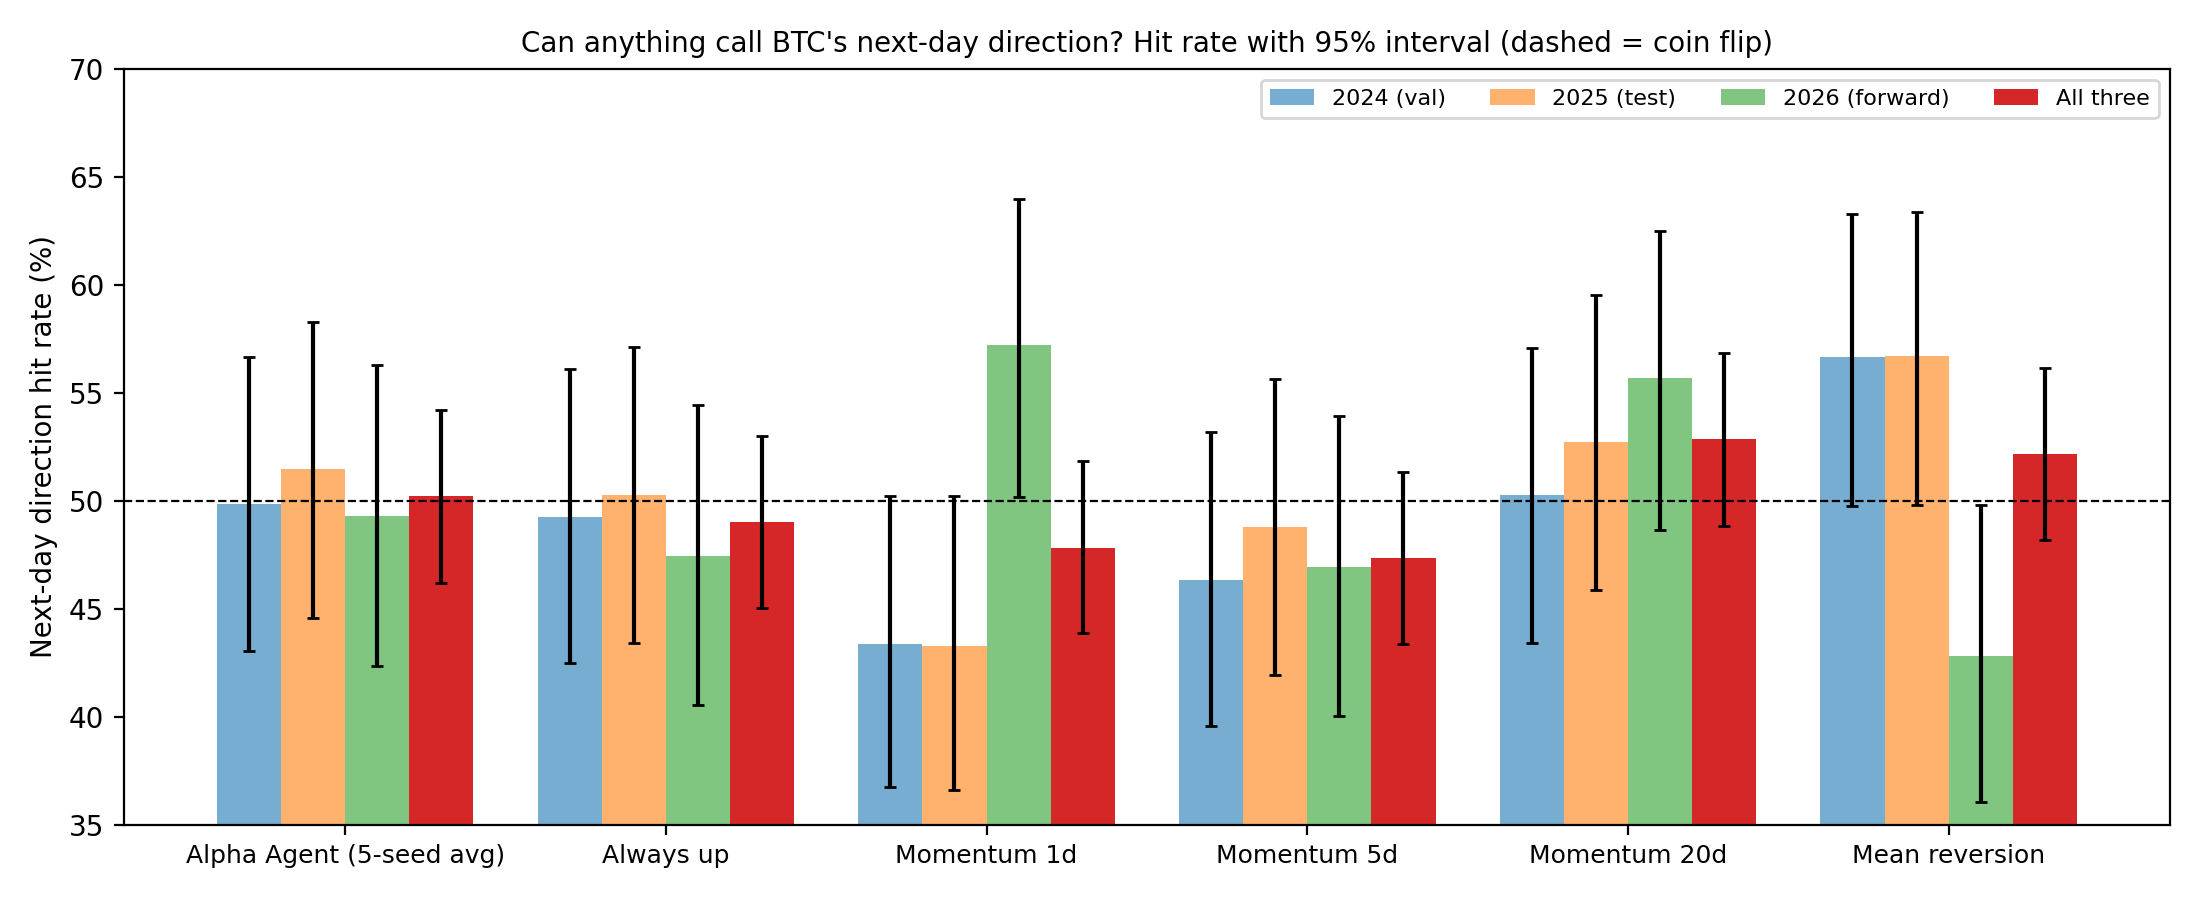
\includegraphics[width=0.9\textwidth]{phase5_direction_baselines.png}
  \caption{Direction hit rates with 95\% intervals; dashed line = 50\%.}
  \label{fig:direction}
\end{figure}

\begin{guide}
Say it plainly: every pooled interval contains 50\%, so neither the Alpha Agent nor any simple rule can be told apart from a coin flip. Rules that looked good in one year reversed in another (mean reversion 57\% $\to$ 43\%), which is what noise looks like. Several model seeds predicted one direction on almost every day.
\end{guide}
\tbc{}

% ---------------------------------------------------------------------
\section{Volatility and jump-risk forecasting}\label{sec:res-vol}

\begin{figure}[ht]
  \centering
  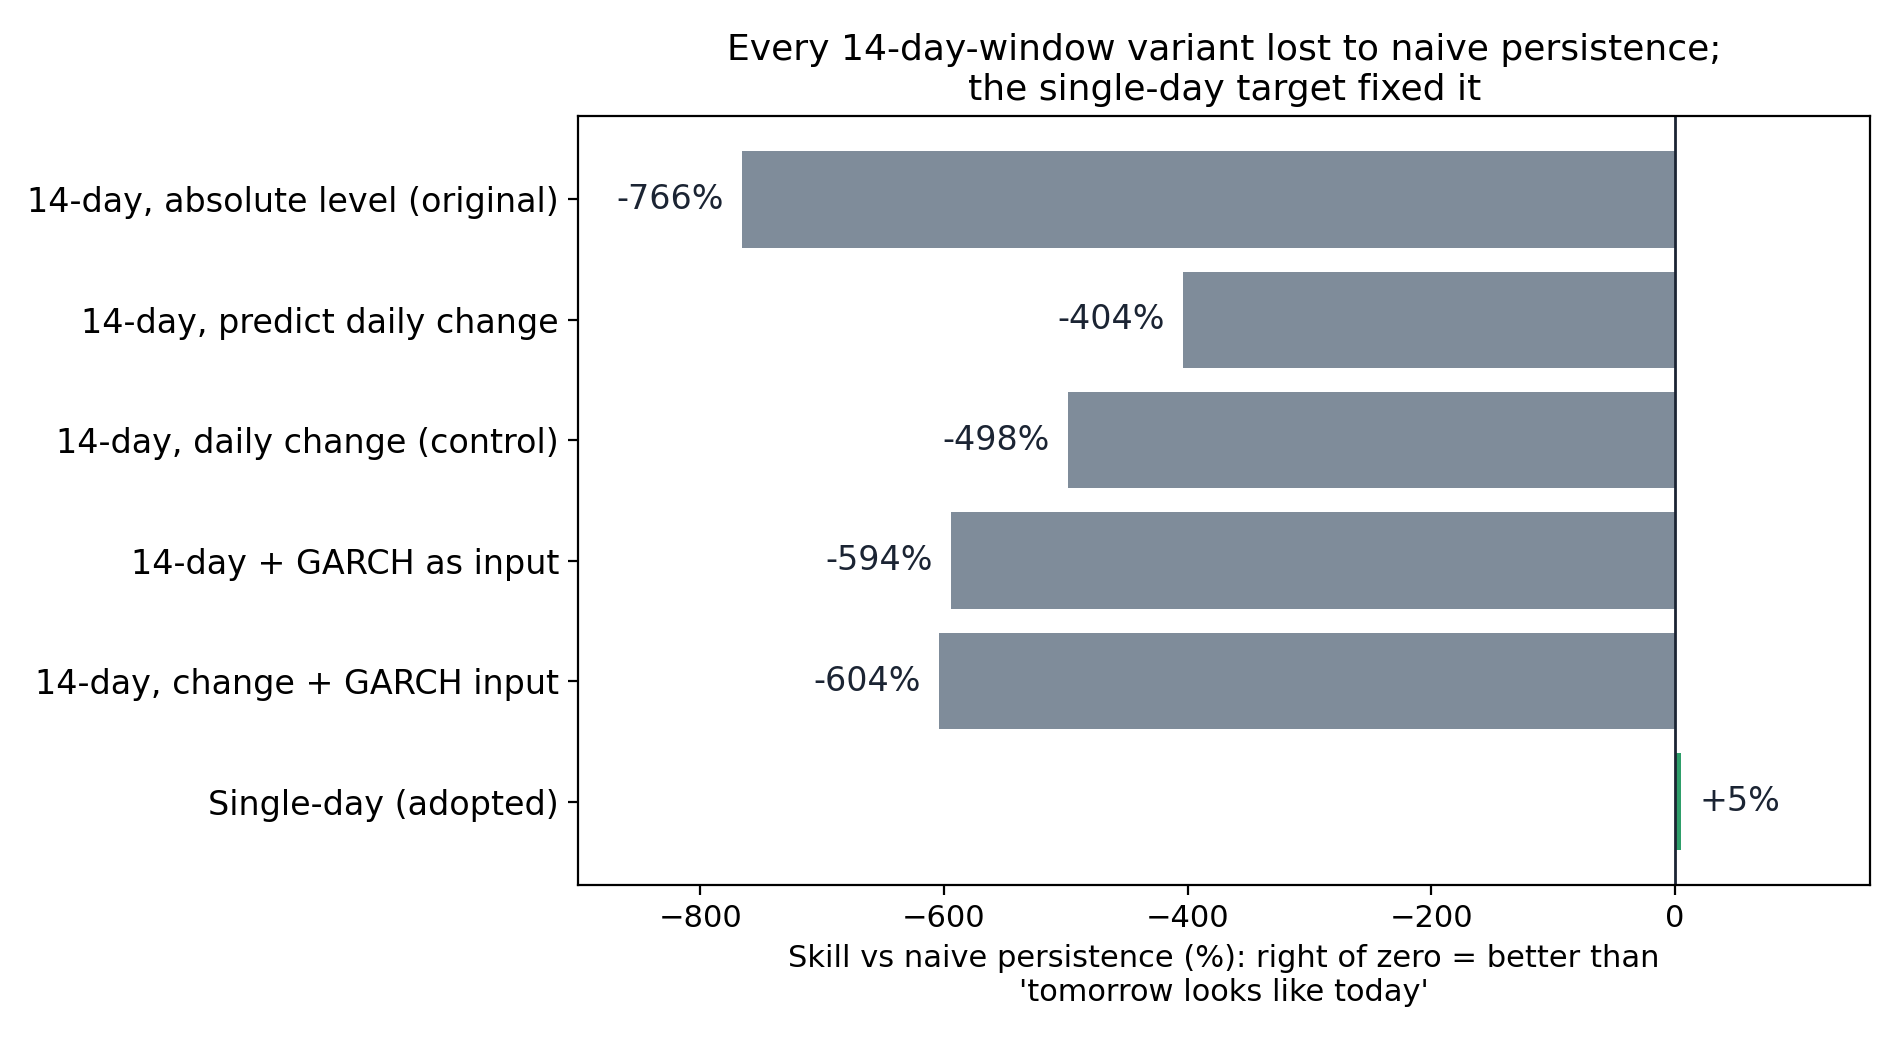
\includegraphics[width=0.8\textwidth]{phase3_volatility_target.png}
  \caption{Skill relative to naive persistence for every volatility-target variant.}
  \label{fig:vol-target}
\end{figure}

\begin{table}[ht]
  \centering
  \caption{Volatility forecast error (RMSE of the size of the next day's move).}
  \label{tab:vol}
  \begin{tabular}{lcc}
    \toprule
    Method & 2025 test & 2026 forward \\
    \midrule
    Naive persistence (today's move) & 0.02079 & 0.02500 \\
    GARCH(1,1)                      & 0.02246 & \tbc{} \\
    Beta Agent                      & 0.01974 & 0.02038 $\pm$ 0.00101 \\
    \bottomrule
  \end{tabular}
\end{table}

\begin{guide}
The Beta Agent beats persistence (5\% lower RMSE in 2025, 18\% in 2026) and GARCH. Be honest about the limits (found 20 Oct): on the backtest days its forecast averaged 3.0\% against an actual average move of 1.78\% - it is biased high, probably because 2018--2023 was more volatile than 2025 - and its correlation with the actual move is only 0.19. It ranks days in the right order, but weakly. The tuned $k$ and $c$ absorb the constant bias, which is why the Risk Engine still benefits. Then report the jump classifier: \tbc{Platt-calibrated jump probability results - AUC / Brier / calibration from Phase 3}.
\end{guide}
\tbc{}

% ---------------------------------------------------------------------
\section{Trading results on the 2025 test (H3)}\label{sec:res-h3}

\begin{table}[ht]
  \centering
  \caption{2025 test backtest, R1{,}000 starting capital, 2x leverage cap (mean $\pm$ std over 5 runs).}
  \label{tab:backtest2025}
  \begin{tabular}{lccc}
    \toprule
    & Dynamic Risk Engine & Fixed rules & Buy \& hold BTC \\
    \midrule
    Final balance     & R1{,}045 $\pm$ 60 & R931 $\pm$ 67 & R1{,}000 \\
    Lowest balance    & R968 $\pm$ 13 & R884 $\pm$ 47 & R872 \\
    Max drawdown      & 4.6\% $\pm$ 1.1 & 17.2\% $\pm$ 3.0 & 31.8\% \\
    Sharpe            & 0.74 $\pm$ 1.09 & $-0.50 \pm 0.59$ & 0.19 \\
    Sortino           & 1.43 $\pm$ 1.84 & $-0.77 \pm 0.90$ & 0.27 \\
    Trades            & 63 & 201 & -- \\
    Liquidations      & 0 & 0 & -- \\
    \bottomrule
  \end{tabular}
\end{table}

\begin{figure}[ht]
  \centering
  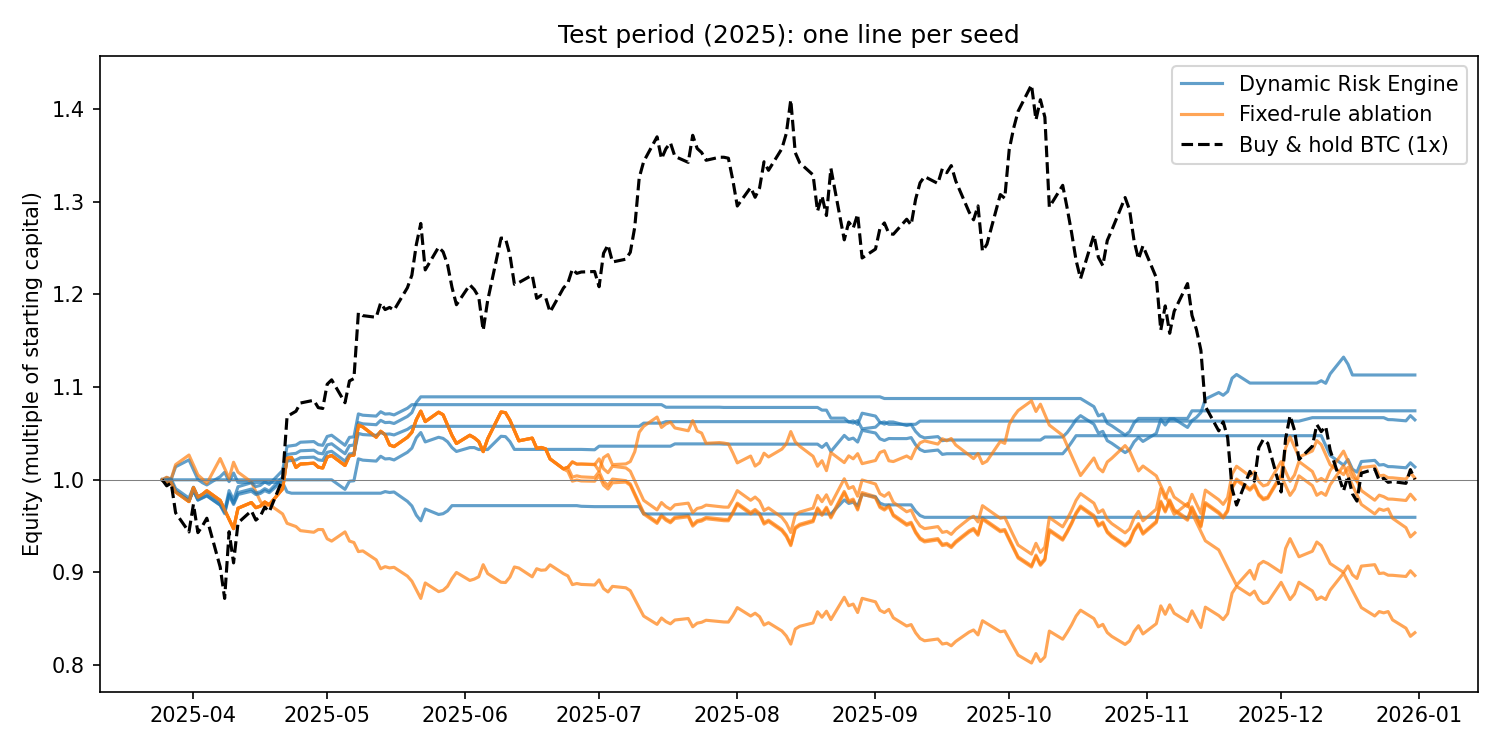
\includegraphics[width=0.9\textwidth]{phase4_equity_curves.png}
  \caption{Account value through 2025.}
  \label{fig:equity2025}
\end{figure}

\subsection{Significance}
\begin{table}[ht]
  \centering
  \caption{Risk Engine minus fixed rules, paired moving-block bootstrap (5{,}000 resamples, 10-day blocks), 5-seed average. Positive = Risk Engine better.}
  \label{tab:bootstrap}
  \begin{tabular}{lccc}
    \toprule
    & Observed & 95\% interval & $p$ (one-sided) \\
    \midrule
    Drawdown reduction (pp), 2025 & +12.6 & [+7.0, +20.9] & $<0.0002$ \\
    Sharpe gain, 2025             & +1.24 & [+0.20, +2.45] & 0.011 \\
    Drawdown reduction (pp), 2026 & +14.1 & [+4.5, +19.2] & $<0.0002$ \\
    Sharpe gain, 2026             & +0.53 & [$-0.44$, +1.65] & 0.139 \\
    \bottomrule
  \end{tabular}
\end{table}

\begin{guide}
Also report the daily-return DM-style test (Newey--West): significant on 0 of 5 seeds - i.e.\ the Risk Engine does not earn significantly more per day; its advantage is in avoiding large losses. Use \texttt{phase5\_h3\_bootstrap.png} if you want a figure.
\end{guide}
\tbc{}

\subsection{Which rules matter?}
\begin{table}[ht]
  \centering
  \caption{Rule-by-rule ablation, 2025 test: each rule replaced by its fixed version and the system retuned.}
  \label{tab:rule-ablation}
  \begin{tabular}{lccc}
    \toprule
    Version & Max drawdown & Extra drawdown (pp) & Sharpe \\
    \midrule
    All five rules             & 4.6\%  & --    & 0.74 \\
    Fixed stop-loss            & 8.2\%  & +3.6  & $-0.14$ \\
    No weak-prediction filter  & 7.9\%  & +3.3  & 0.39 \\
    Fixed position size        & 6.8\%  & +2.2  & 0.71 \\
    No jump veto               & 5.6\%  & +1.0  & 0.47 \\
    Fixed leverage             & 4.9\%  & +0.3  & 0.74 \\
    All fixed (H3 ablation)    & 17.2\% & +12.6 & $-0.50$ \\
    \bottomrule
  \end{tabular}
\end{table}
\tbc{figure: phase5\_rule\_ablation.png; point: no one rule carries the result, together they matter a lot; the volatility stop matters most}

\subsection{Does the direction model matter?}
\begin{table}[ht]
  \centering
  \caption{Swapping the direction forecaster inside the full framework (2025 test).}
  \label{tab:model-ablation}
  \begin{tabular}{lcccc}
    \toprule
    Forecaster & Max drawdown & Sharpe & Final balance & Hit rate \\
    \midrule
    Alpha Agent (attention) & 4.6\% & 0.74 & R1{,}045 & 51.4\% \\
    Bi-LSTM, no attention   & 3.4\% & 0.36 & R1{,}010 & 50.7\% \\
    Univariate LSTM         & 9.2\% & $-0.44$ & R973 & 53.6\% \\
    \bottomrule
  \end{tabular}
\end{table}
\tbc{none of the differences is significant (Alpha vs Bi-LSTM: $p = 0.87$ drawdown, $0.35$ Sharpe; vs univariate LSTM: $p \approx 0.10$ for both)}

\subsection{Leverage stress test}
\begin{table}[ht]
  \centering
  \caption{2025 test at higher leverage caps, both engines retuned on 2024 at each cap.}
  \label{tab:stress}
  \small
  \begin{tabular}{ccccc}
    \toprule
    Cap & MDD Risk Engine & MDD fixed & Balance Risk Engine & Liquidations (RE / fixed) \\
    \midrule
    2x  & 4.6\%  & 17.2\% & R1{,}045 & 0 / 0 \\
    5x  & 12.6\% & 38.3\% & R1{,}106 & 0 / 0 \\
    10x & 24.2\% & 42.2\% & R1{,}214 & 0 / 0 \\
    20x & 38.2\% & 68.8\% & R1{,}500 & 2 / 0 \\
    \bottomrule
  \end{tabular}
\end{table}

\begin{guide}
Drawdown reduction is significant at every cap ($p<0.0002$). The liquidation part of H3 is NOT supported: below 20x neither engine was ever liquidated (a stop tighter than $1/L$ always fires first), and at 20x the Risk Engine was liquidated twice because its volatility-widened stops sat beyond the 5\% liquidation line. Figure: \texttt{phase5\_leverage\_stress.png}.
\end{guide}
\tbc{}

% ---------------------------------------------------------------------
\section{Forward test on unseen 2026 data}\label{sec:res-forward}

\begin{table}[ht]
  \centering
  \caption{1 January -- 30 September 2026 (194 trading days). Nothing retrained or retuned.}
  \label{tab:forward}
  \begin{tabular}{lccc}
    \toprule
    & Dynamic Risk Engine & Fixed rules & Buy \& hold BTC \\
    \midrule
    Final balance  & R1{,}024 $\pm$ 86 & R986 $\pm$ 196 & R942 \\
    Lowest balance & R943 $\pm$ 57 & R835 $\pm$ 120 & R660 \\
    Max drawdown   & 8.7\% $\pm$ 3.8 & 22.8\% $\pm$ 6.4 & 39.6\% \\
    Sharpe         & 0.35 $\pm$ 1.02 & $-0.18 \pm 1.39$ & 0.04 \\
    Liquidations   & 0 & 0 & -- \\
    \bottomrule
  \end{tabular}
\end{table}

\begin{figure}[ht]
  \centering
  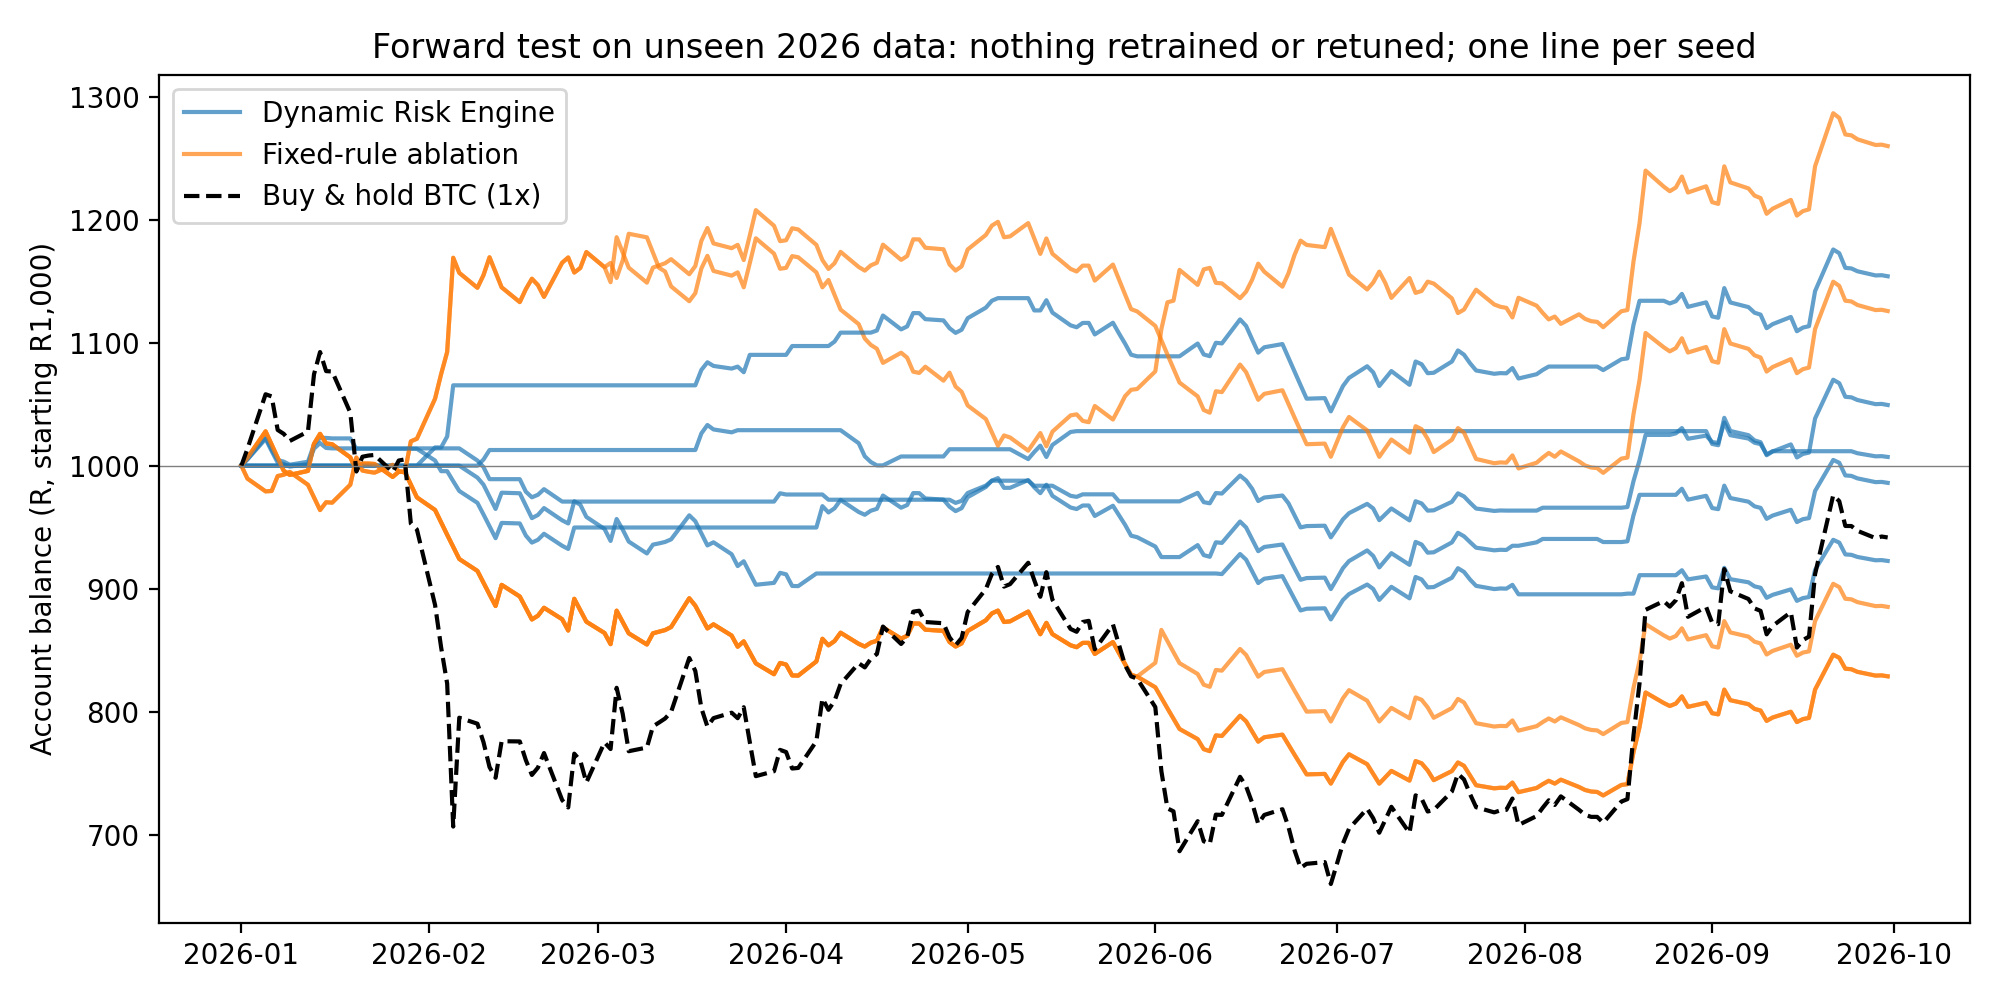
\includegraphics[width=0.9\textwidth]{phase5_forward_2026.png}
  \caption{Account value through the 2026 forward period.}
  \label{fig:forward}
\end{figure}

\begin{guide}
This is your cleanest evidence: the drawdown result replicated on data that did not exist when the system was built. Alpha hit rate 49.3\% (coin flip again); Beta RMSE 0.0204 vs persistence 0.0250. Optionally add the leverage menu (\texttt{phase5\_forward\_2026\_leverage.png}: 2x +2.4\%, 5x +5.6\%, 10x +9.1\%, 20x $-12.1\%$ average return; Sharpe roughly flat until it collapses at 20x) - present it as ``more leverage widens outcomes, it does not improve return per unit of risk''.
\end{guide}
\tbc{}

\section{Summary of hypotheses}
\begin{table}[ht]
  \centering
  \caption{Outcome for each hypothesis.}
  \label{tab:scorecard}
  \begin{tabularx}{\textwidth}{lX}
    \toprule
    Hypothesis & Outcome \\
    \midrule
    H1 & Partly supported: lower RMSE on average, but not consistent across seeds. \\
    H2 & Partly supported: attention helps only when the plain Bi-LSTM trains unstably; no measurable effect in trading. \\
    H3 & Drawdown: strongly supported (2025 and 2026, every leverage cap). Risk-adjusted return: not worse, better on average (significant in 2025, not in 2026). Liquidations: not supported. \\
    \bottomrule
  \end{tabularx}
\end{table}
